\documentclass[11pt]{article}
\usepackage{evals}
\usepackage{mathtools} 
\usepackage{fancyvrb}

\def \autores {F. Milanese, M.Solano, M.Vega.}
\def \semestre {2016-2}
\def \titulo {Cert\'amen 1, C\'alculo Num\'erico 525230}
\def \fecha {Pauta (la primera alternativa es la correcta)}


\title{C1R-NUMERICO}

\begin{document}
\encabezado{encabezado.tex}{1}

\begin{pregunta}
\puntaje{5}
\begin{cuerpo}
Sobre la función de la forma
$$
f(x)=e^{ax^2+bx}
$$
que mejor se ajusta a los puntos 
$\{(-1,1),(1,1),(0,1)\}$, es correcto afirmar que
\end{cuerpo}
\begin{alternativas}
{Es un polinomio interpolante.} %Siempre la primera es la correcta
{Es $e^{x^2+x}$.}
{Es una parábola.}
{No se puede calcular.}
\end{alternativas}
\justificacion{7cm}
\end{pregunta}

\begin{pregunta}
\puntaje{5}
\begin{cuerpo}
La gráfica 
\begin{center}
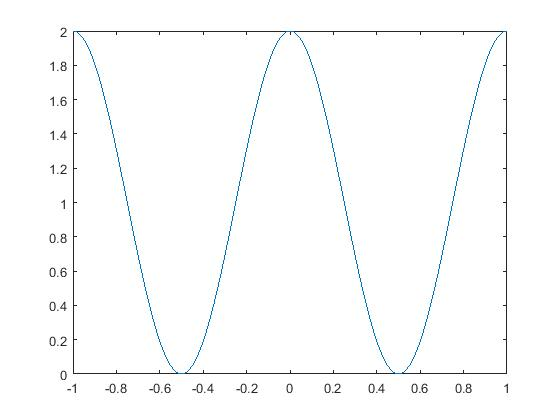
\includegraphics[width=0.5\textwidth]{./img/img1.jpg}
\end{center}
se genera con las instrucciones
\end{cuerpo}
\begin{multicols}{2}
\begin{alternativas}
{\texttt{
x=-1:0.01:1; \\
y=cos(2*pi*x)+1; \\
plot(x,y);}}
{\texttt{
x=-1:0.01:1; \\
y=cos(2*pi*x); \\
plot(x,y);}\\} 
{\texttt{
x=-1:0.01:1; \\
y=sin(2*pi*x)+1; \\
plot(x,y);}}
{\texttt{
plot(cos(x)+1);}}
\end{alternativas}
os\end{multicols}
\justificacion{0cm}
\end{pregunta}
\begin{pregunta}
\puntaje{5}
\begin{cuerpo}
Sobre la representación de números en punto flotante se establecen las siguientes proposiciones
\begin{enumerate}
\item[i)] es capaz de registrar sin error cualquier entero.
\item[ii)] siempre que representa un número comete un error de redondeo.
\item[iii)] es capaz de representar irracionales sin errores.
\end{enumerate}
Es correcto afirmar que
\end{cuerpo}
\begin{multicols}{2}
\begin{alternativas}
{i), ii) y iii) son falsas.} %Siempre la primera es la correcta
{Sólo i) y iii) son falsas..}
{Sólo ii) es verdadera.}
{Sólo i) es verdadera.}
\end{alternativas}
\end{multicols}
\justificacion{0cm}
\end{pregunta}
\begin{pregunta}
\begin{cuerpo}
El P.V.I.
$$
Li''(t)+Ri'(t)+\frac{1}{C}i(t)=0
$$
modela la corriente $i(t)[A]$ en un circuito de resistencias, bobinas y condensadores (RLC) de resistencia $R[\Omega]$, capacitancia $C[F]$ e inductancia $L[H]$. Cu\'al de las siguientes funciones de Matlab grafica la soluci\'on de este problema para distintos datos de $RLC$ y condiciones iniciales.
\end{cuerpo}

\begin{multicols}{2}
\begin{alternativas}
{
\texttt{function rlc(R,L,C,i0,di0)}\\
\texttt{f=@(t,u) [u(2);-R/L*u(2)-1/(L*C)*u(1)];}\\
\texttt{[t,u]=ode45(f,[0,100],[i0;di0]);}\\
\texttt{plot(t,u(:,1))}		}
{
\texttt{function rlc(R,L,C,i0,di0)}\\
\texttt{f=@(t,u) [u(2);-R/L*u(2)-1/(L*C)*u(1)];}\\
\texttt{[t,u]=ode45(f,[i0;di0],[0,100]);}\\
\texttt{plot(t,u(:,1))}		}
{
\texttt{function rlc(R,L,C,i0,di0)}\\
\texttt{f=@(t,u) [u(2);-R/L*u(2)-1/(L*C)*u(1)];}\\
\texttt{[t,u]=ode45(f,[0,100],[i0;di0]);}\\
\texttt{plot(t,u(:,2))}		}
{
\texttt{function rlc(R,L,C,i0,di0)}\\
\texttt{f=@(t,u) [u(2);-R*u(2)-1/C*u(1)];}\\
\texttt{[t,u]=ode45(f,[0,100],[i0;di0]);}\\
\texttt{plot(t,u(:,1))}		}
\end{alternativas}
\end{multicols}
\justificacion{0cm}
\end{pregunta}
\begin{pregunta}
\begin{cuerpo}
Aproximar la siguiente integral utilizando la regla elemental del punto medio en la direcci\'on $x$ y la regla elemental de simpson en la direcci\'on $y$.
$$
\int_0^1 \int_0^\pi \frac{\cos(2x)}{y+1} dx\,dy.
$$
\end{cuerpo}
\begin{multicols}{4}
\begin{alternativas}
{$-\frac{25}{36}\pi$} %Siempre la primera es la correcta
{$\frac{2}{3}\pi$} 
{$0$} 
{$\frac{\pi}{6}\left(1+\frac{4}{\frac{\pi}{2}+1}+\frac{1}{\pi+1}\right)$}
\end{alternativas}
\end{multicols}
\justificacion{7cm}
\end{pregunta}

\begin{pregunta}
%\puntaje{5}
\begin{cuerpo}
Se aproxim\'o una de las ra\'ices de la funci\'on $f(x)= x^2-9$ con tres m\'etodos num\'ericos diferentes. Para cada uno de ellos se utilizaron valores iniciales cercanos a la soluci\'on o intervalos apropiados, obteni\'endose las siguientes aproximaciones de la ra\'iz buscada:
\begin{center}
\begin{tabular}{c||c|c|c}
N$^\circ$ de iteraciones & M\'etodo A & M\'etodo B & M\'etodo C  \\
\hline \hline
$1$ & $3.2195$&$3.0500$& $3.2500$  \\
$2$ & $2.9579$&$2.5750$& $3.0096$     \\
$3$ & $2.9985$&$2.8125$& $3.0000$   \\
$4$ & $3.0000$&$2.9312$& $3.0000$ \\   
$5$ & $3.0000$&$2.9906$& $3.0000$ \\ 
\end{tabular}
\end{center}
?`Cuales son estos m\'etodos?
\end{cuerpo}

\begin{alternativas}
{M\'etodo A: M\'etodo de la Secante. M\'etodo B: M\'etodo de la Bisecci\'on. M\'etodo C:  Newton-Raphson.}  %Siempre la primera es la correcta
{M\'etodo A: Newton-Raphson. M\'etodo B: M\'etodo de la Secante. M\'etodo C: M\'etodo de la Bisecci\'on.}
{M\'etodo A: M\'etodo de la Bisecci\'on. M\'etodo B:  Newton-Raphson. M\'etodo C: M\'etodo de la Secante.} 
{M\'etodo A: M\'etodo de la Bisecci\'on. M\'etodo B: M\'etodo de la Secante. M\'etodo C:  Newton-Raphson.}
\end{alternativas}
\justificacion{7cm}
\end{pregunta}
\begin{pregunta}
\begin{cuerpo}
Considere el siguiente problema de valores iniciales:
\begin{eqnarray*}
\left \{
\begin{array}{lcl}
y'(x)&=& \cos(x)y(x) + x^3, \quad  x \in [0,1]\\
y(0)&=&0.
\end{array}
\right.
\end{eqnarray*}
Se utiliza el m\'etodo de Euler Expl\'icito con tama\~no de paso uniforme $h=1/4$ para aproximar la soluci\'on de este problema. ?`C\'ual de los siguientes valores corresponde a $y_2$ (aproximaci\'on de $y(x)$ en $x_2$)? 
\end{cuerpo}
\begin{multicols}{4}
\begin{alternativas}
{$\displaystyle\frac{1}{4^4}$} %Siempre la primera es la correcta
{{$\displaystyle\frac{\pi^3}{4^4}$}} 
{$0$} 
{$\displaystyle\frac{1}{4^3}$}
\end{alternativas}
\end{multicols}
\justificacion{7cm}
\end{pregunta}

\begin{pregunta}
\puntaje{}
\begin{cuerpo}
Considere los siguientes puntos $(x_0,y_0), (x_1,y_1), \ldots, (x_n,y_n)$, con $n\geq2$ e $0<y_i<1$, para todo $i=0,1,\ldots, n$. Estos puntos se ajustan en el sentido de los m\'inimos cuadrados al modelo $f(t)=\dfrac{1}{\beta e^{\alpha t}+1}$, $t\in [a,b]$, donde $\alpha$ y $\beta$ son par\'ametros a determinar.

Considere las siguientes funciones de Matlab.\medskip

\hspace{-1.25in}
\begin{minipage}{1.15\textwidth}
\begin{multicols}{2}
\begin{itemize}
\item[i)] \hspace{0.025\textwidth}
\begin{minipage}{0.4\textwidth}
\begin{lstlisting}
function [alfa,beta] = mincuad(x,y,a,b)
A = [ones(length(x),1) x];
B = log(1./y-1);
X = A \ B;
beta = exp(X(1));
alfa = X(2);
t = linspace(a,b,100);
z = 1./(beta.*exp(alfa.*t)+1);
plot(x,y,'o',t,z);
\end{lstlisting}
\end{minipage}

\item[ii)] \hspace{0.025\textwidth}
\begin{minipage}{0.4\textwidth}
\begin{lstlisting}
function [alfa,beta] = mincuad(x,y,a,b)
A = [ones(length(x),1) x];
B = log(1./y-1);
X = A \symbol{`\\} B;
beta = X(1);
alfa = X(2);
t = linspace(a,b,100);
z = 1./(beta.*exp(alfa.*t)+1);
plot(x,y,'o',t,z);
\end{lstlisting}
\end{minipage}

\item[iii)] \hspace{0.025\textwidth}
\begin{minipage}{0.4\textwidth}
\begin{lstlisting}
function [alfa,beta] = mincuad(x,y,a,b)
A = [ones(length(x),1) x];
B = log(1./y-1);
X = A \symbol{`\\} B;
beta = exp(X(1));
alfa = X(2);
t = linspace(a,b,100);
z = beta + alfa.*t;
plot(x,y,'o',t,z);
\end{lstlisting}
\end{minipage}

\item[iv)] \hspace{0.025\textwidth}
\begin{minipage}{0.4\textwidth}
\begin{lstlisting}
function [alfa,beta] = mincuad(x,y,a,b)
A = [ones(length(x),1) x];
B = y;
X = A \symbol{`\\} B;
beta = X(1);
alfa = X(2);
t = linspace(a,b,100);"
z = beta + alfa.*t;"
plot(x,y,'o',t,z);
\end{lstlisting}
\end{minipage}

\end{itemize}
\end{multicols}

\end{minipage}
\end{cuerpo}
\bigskip

 ?`Cu\'al o c\'uales de estas funciones en Matlab grafica los puntos y la funci\'on $f(t)$?
 
\begin{multicols}{2}
\begin{alternativas}
{S\'olo i)} %Siempre la primera es la correcta
{S\'olo ii)}
{S\'olo iii)}
{S\'olo i) y iv)}
\end{alternativas}
\end{multicols}
\justificacion{0cm}
\end{pregunta}

\begin{pregunta}
\begin{cuerpo}
Considere la funci\'on
$$
\displaystyle
f(x)=\int_0^x cos^2(2t+1) dt\quad,
$$
sobre la b\'usqueda de ra\'ices positivas de $f$, es siempre cierto que
\end{cuerpo}
\begin{alternativas}
{No se puede ejecutar el m\'etodo de la bisecci\'on para esta funci\'on.}
{El m\'etodo de Newton Raphson converger\'a para cualquier aproximaci\'on inicial.}
{El m\'etodo de la bisecci\'on encontrar\'a algunas ra\'ices de $f$.}
{El m\'etodo de Newton Raphson converger\'a mas r\'apido que el de la secante.}
\end{alternativas}
\justificacion{0cm}
\end{pregunta}
\begin{pregunta}
\begin{cuerpo}
Considere el siguiente sistema de ecuaciones
$$
\left(\begin{array}{rrr}
-2&2&0\\
2&-2&1\\
0&1&0\\
\end{array}\right)
\left(\begin{array}{r}
x_1\\
x_2\\
x_3
\end{array}\right)
=
\left(\begin{array}{r}
1\\
2\\
3\\
\end{array}\right).
$$
>Cu\'al de los siguientes m\'etodos es el m\'as eficiente para resolver el sistema anterior?
\end{cuerpo}
\begin{alternativas}
{La factorizaci\'on LU \textbf{con estrategia de pivoteo parcial}.}
{El m\'etodo de eliminaci\'on Gaussiana \textbf{sin estrategia de pivoteo parcial}.}
{El algoritmo de Thomas, aprovechando \textbf{la estructura tridiagonal} de la matriz de coeficientes.}
{La factorizaci\'on de Cholesky, aprovechando que la matriz de coeficientes es \textbf{sim\'etrica y definida positiva}.}
\end{alternativas}
\justificacion{0cm}
\end{pregunta}
\begin{pregunta}
\begin{cuerpo}
Considere la siguiente tabla de datos:

\bigskip
\begin{center}
\begin{tabular}{r||r|r|r|r|r}
$x_i$&$-1$&0&1&2&4\\
\hline
$y_i$&1&$-1$&1&$-1$&1
\end{tabular}
\qquad con $i=0,1,2,3,4$
\end{center}
\bigskip

y $l_0(x)$, $l_1(x)$, $l_2(x)$, $l_3(x)$ y $l_4(x)$ sus respectivos polinomios de Lagrange. Indique cu\'al de las siguientes afirmaciones es \textbf{siempre verdadera}.
\end{cuerpo}
\begin{alternativas}
{Existen $\alpha_i\in \mathbb{R}$, con $i=0,\ldots,4$, tales que $x^3-1=\displaystyle \sum_{i=0}^4\alpha_il_i(x)$}
{El polinomio $p(x)=-l_0(x)+l_2(x)+2l_3(x)+4l_4(x)$ interpola a los puntos de la tabla.}
{Los puntos de la tabla no pueden ser interpolados por una spline c\'ubica natural.}
{Existen dos polinomios $q$ y $r$ de grado menor o igual a 4 tales que $q(x_i)=r(x_i)=y_i$, para todo $i=0,\ldots,4$, pero que $q(x)\neq r(x)$, para alg\'un $x\in\mathbb{R}$.}
\end{alternativas}
\justificacion{0cm}
\end{pregunta}
\begin{pregunta}
\begin{cuerpo}
Considere la siguiente matriz:

$$\boldsymbol{A}=\left(
\begin{array}{rrr}
2&-3&1\\
3&2&2\\
1&3&2
\end{array}
\right)
$$

>Cu\'al de las siguientes matrices corresponde a la matriz de permutaci\'on de la factorizaci\'on $\boldsymbol{PA}=\boldsymbol{LU}$, con $\boldsymbol{L}$ triangular inferior y $\boldsymbol{U}$ triangular superior?
\end{cuerpo}
\begin{multicols}{2}
\begin{alternativas}
{$\displaystyle\boldsymbol{P}=\left(\begin{array}{rrr} 0&1&0\\ 1&0&0\\ 0&0&1 \end{array}\right)$}
{$\displaystyle\boldsymbol{P}=\left(\begin{array}{rrr} 1&0&0\\ 0&1&0\\ 0&0&1 \end{array}\right)$}
{$\displaystyle\boldsymbol{P}=\left(\begin{array}{rrr} 0&0&1\\ 1&0&0\\ 0&1&0 \end{array}\right)$}
{$\displaystyle\boldsymbol{P}=\left(\begin{array}{rrr} 0&1&0\\ 0&0&1\\ 1&0&0 \end{array}\right)$}
\end{alternativas}
\end{multicols}
\justificacion{7cm}
\end{pregunta}
\null\hfill\autores
\end{document}    